\begin{frame}{FSEA results}

    \textbf{Details}
    \begin{itemize}
        \item Feature set enrichment analysis on Neuroactive gene sets
        \item Using all kids
        \item Using Mann-Whitney U test
        \item Adjusted q via Benjamini-Hochberg FDR correction
    \end{itemize}
\end{frame}

\begin{frame}{FSEA results}

    \begin{table}
        \tiny
            \begin{tabular}{rrrrrrr}
              \hline\hline
              \textbf{geneset} & \textbf{U} & \textbf{median} & \textbf{mu} & \textbf{sigma} & \textbf{pvalue} & \textbf{qvalue} \\
              \texttt{String} & \texttt{Float64} & \texttt{Float64} & \texttt{Float64} & \texttt{Float64} & \texttt{Float64} & \texttt{Float64} \\\hline
              Menaquinone synthesis & 1.80593e8 & -0.0227227 & -5.30723e7 & 9.7112e6 & 4.62758e-8 & 1.38827e-6 \\
              Propionate degradation & 7.8577e6 & -0.0520019 & -1.03042e7 & 2.70742e6 & 0.000141289 & 0.00211934 \\
              GABA synthesis & 2.3124e7 & -0.0302445 & -1.31996e7 & 3.82886e6 & 0.000566035 & 0.00424526 \\
              Glutamate degradation & 1.89577e7 & -0.0376948 & -1.25228e7 & 3.56448e6 & 0.000442716 & 0.00424526 \\
              Tryptophan synthesis & 2.56154e8 & -0.00604063 & -2.71454e7 & 1.0693e7 & 0.0111292 & 0.0667749 \\
              S-Adenosylmethionine synthesis & 6.5944e7 & -0.0124222 & -1.39665e7 & 5.67907e6 & 0.013921 & 0.069605 \\
              Acetate synthesis & 2.1512e8 & -0.0140563 & -2.09669e7 & 9.76138e6 & 0.0317181 & 0.135935 \\
              p-Cresol synthesis & 3.26509e7 & -0.0356679 & -8.51573e6 & 4.07613e6 & 0.0366924 & 0.137596 \\
              Quinolinic acid degradation & 1.47932e8 & -0.0163907 & -1.55163e7 & 8.12206e6 & 0.0560839 & 0.168252 \\
              Butyrate synthesis & 4.44021e7 & -0.0320785 & -8.87212e6 & 4.63697e6 & 0.0557039 & 0.168252 \\\hline\hline
            \end{tabular}
          \end{table}

\end{frame} 

\begin{frame}{FSEA results}

    \textbf{Details}
    \begin{itemize}
        \item Feature set enrichment analysis on Neuroactive gene sets
        \item Using all kids with brain scans
        \item Using Mann-Whitney U test
        \item Adjusted q via Benjamini-Hochberg FDR correction
    \end{itemize}
\end{frame}

\begin{frame}{FSEA results}

    \begin{table}
        \tiny
        \begin{tabular}{rrrrr}
            \hline\hline
            \textbf{region} & \textbf{geneset} & \textbf{U} & \textbf{pvalue} & \textbf{qvalue} \\
            \texttt{Symbol} & \texttt{String} & \texttt{Float64} & \texttt{Float64} & \texttt{Float64} \\\hline
            Right Cerebellum White Matter & Menaquinone synthesis & 7.74978e7 & 1.85854e-6 & 0.00135302 \\
            Left Cerebellum White Matter & Menaquinone synthesis & 8.21281e7 & 8.03345e-5 & 0.0194945 \\
            Left Caudate & GABA synthesis & 7.43746e6 & 6.34299e-5 & 0.0194945 \\
            Right Cerebellum White Matter & GABA synthesis & 7.97035e6 & 0.000170094 & 0.0247657 \\
            Right Cerebellum Cortex & Menaquinone synthesis & 8.30886e7 & 0.000161753 & 0.0247657 \\
            Right Cerebellum Cortex & GABA synthesis & 8.1275e6 & 0.000225155 & 0.0273189 \\
            Left Cerebellum Cortex & GABA synthesis & 8.63868e6 & 0.000542555 & 0.0529034 \\
            Left Hippocampus & Menaquinone synthesis & 8.4953e7 & 0.000581357 & 0.0529034 \\
            Brain Stem & Menaquinone synthesis & 8.55193e7 & 0.000839954 & 0.0679429 \\
            Left Hippocampus & GABA synthesis & 9.08537e6 & 0.00112323 & 0.0817708 \\
            Left Cerebellum White Matter & GABA synthesis & 9.24701e6 & 0.00144799 & 0.0921011 \\
            Left Amygdala & GABA synthesis & 9.31564e6 & 0.00161044 & 0.0921011 \\
            Right Accumbens area & Histamine synthesis & 8.48778e5 & 0.00164466 & 0.0921011 \\
            Right Cerebellum White Matter & Glutamate degradation & 1.01619e7 & 0.00195892 & 0.101864 \\
            Left Amygdala & Glutamate synthesis & 4.84973e7 & 0.00230519 & 0.102444 \\
            Right Cerebellum White Matter & Inositol degradation & 3.41852e6 & 0.00253296 & 0.102444 \\
            Brain Stem & Glutamate synthesis & 7.48954e7 & 0.00215846 & 0.102444 \\
            CSF & Menaquinone synthesis & 1.21243e8 & 0.00249003 & 0.102444 \\
            Left Cerebellum White Matter & Inositol degradation & 3.71948e6 & 0.0046878 & 0.126397 \\
            Left Putamen & GABA synthesis & 1.00288e7 & 0.00461295 & 0.126397 \\
            Left Pallidum & GABA synthesis & 9.86761e6 & 0.00366688 & 0.126397 \\
            Left Amygdala & Tryptophan synthesis & 1.22323e8 & 0.00346543 & 0.126397 \\
            Right Lateral Ventricle & p-Cresol synthesis & 2.70358e7 & 0.00388996 & 0.126397 \\
            Right Caudate & GABA synthesis & 1.0038e7 & 0.00467257 & 0.126397 \\
            Right Putamen & Glutamate synthesis & 7.39107e7 & 0.00451969 & 0.126397 \\
            Right Accumbens area & Glutamate synthesis & 7.40534e7 & 0.00407287 & 0.126397 \\
            CSF & Butyrate synthesis & 3.86017e7 & 0.00389266 & 0.126397 \\
            Left Accumbens area & ClpB & 2.99465e7 & 0.00541846 & 0.14088 \\
            Right Accumbens area & Butyrate synthesis & 3.80803e7 & 0.00666094 & 0.167213 \\
            Right Cerebellum White Matter & Propionate degradation & 2.00749e6 & 0.00742702 & 0.180229 \\\hline\hline
        \end{tabular}
    \end{table}

\end{frame} 


\begin{frame}{Menaquinone synthesis}
    \begin{columns}[c] % The "c" option specifies centered vertical alignment while the "t" option is used for top vertical alignment

        \column{.7\textwidth} % Right column and width
        \begin{figure}
            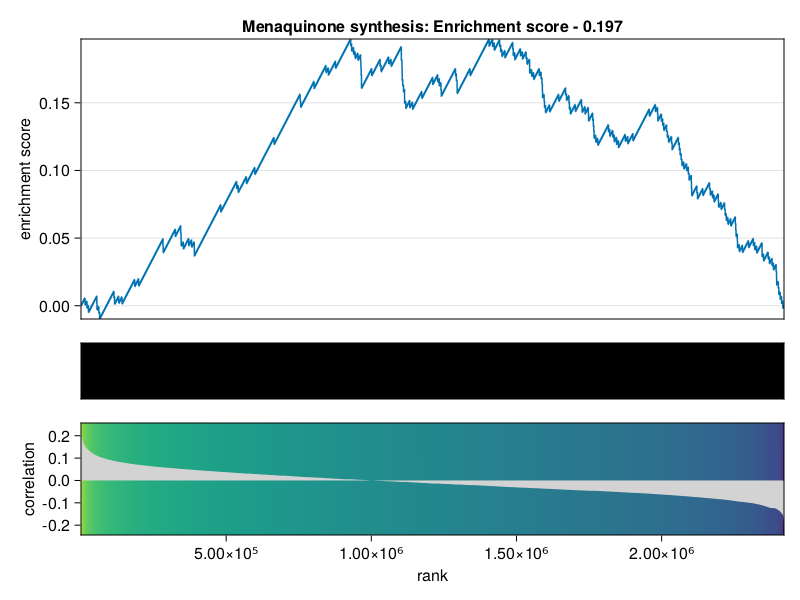
\includegraphics[width=1\linewidth]{../figures/fsea_Menaquinone-synthesis.png}
        \end{figure}

    \end{columns}

\end{frame}

\begin{frame}{Propionate degradation}
    \begin{columns}[c] % The "c" option specifies centered vertical alignment while the "t" option is used for top vertical alignment

        \column{.7\textwidth} % Right column and width
        \begin{figure}
            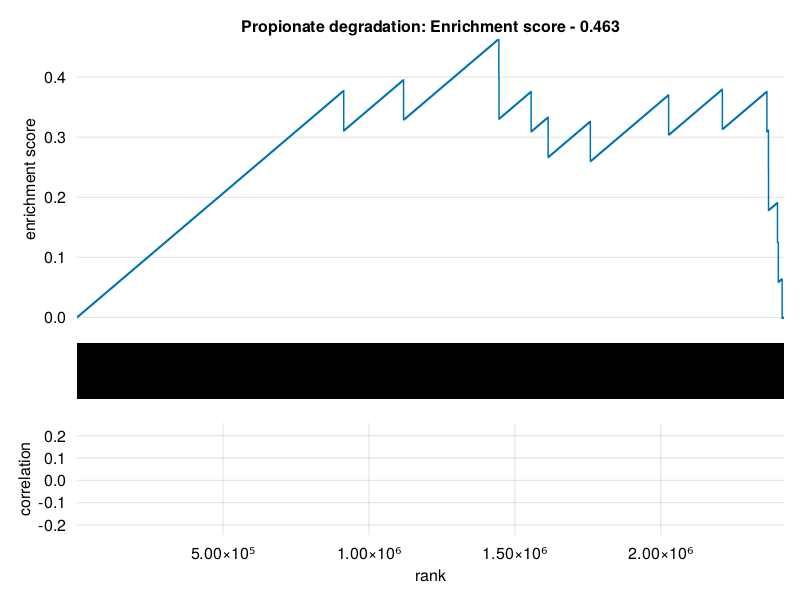
\includegraphics[width=1\linewidth]{../figures/fsea_Propionate-degradation.png}
        \end{figure}

    \end{columns}

\end{frame}

\begin{frame}{Glutamate degradation}
    \begin{columns}[c] % The "c" option specifies centered vertical alignment while the "t" option is used for top vertical alignment

        \column{.7\textwidth} % Right column and width
        \begin{figure}
            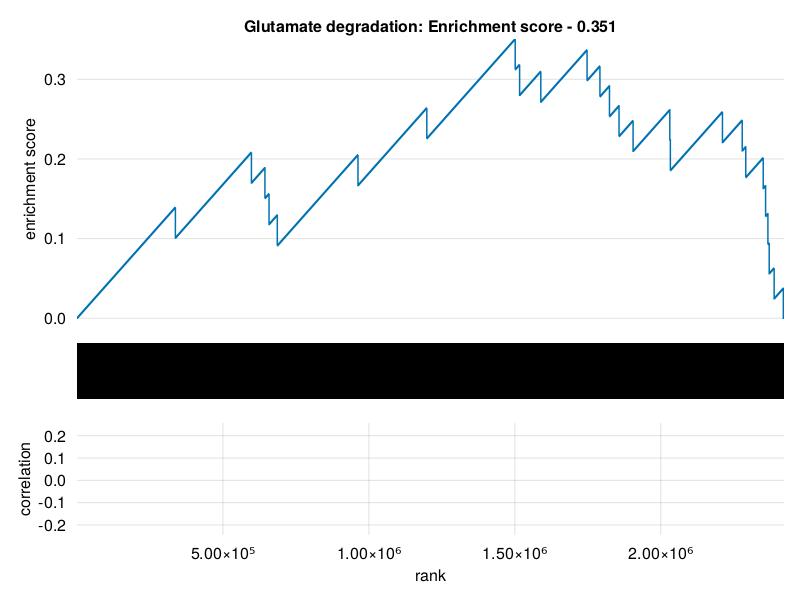
\includegraphics[width=1\linewidth]{../figures/fsea_Glutamate-degradation.png}
        \end{figure}

    \end{columns}

\end{frame}

\begin{frame}{GABA synthesis}
    \begin{columns}[c] % The "c" option specifies centered vertical alignment while the "t" option is used for top vertical alignment

        \column{.7\textwidth} % Right column and width
        \begin{figure}
            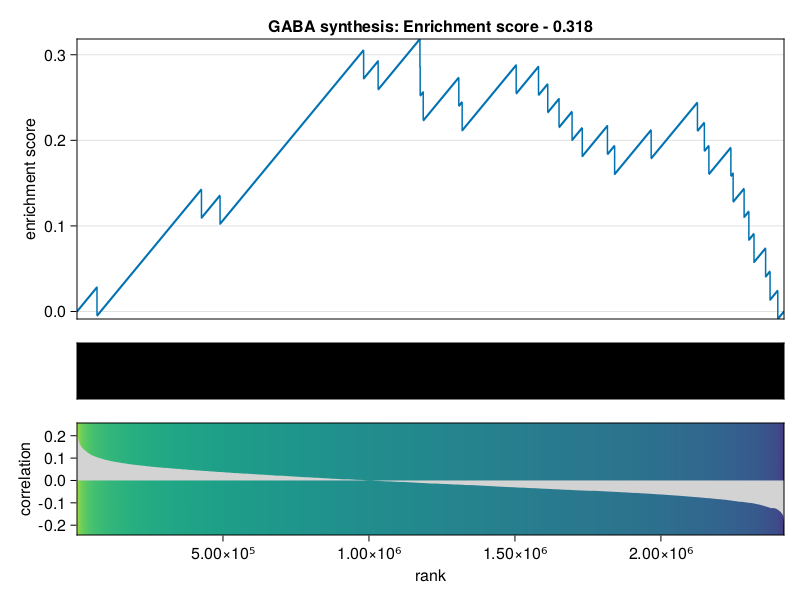
\includegraphics[width=1\linewidth]{../figures/fsea_GABA-synthesis.png}
        \end{figure}

    \end{columns}

\end{frame}

\begin{frame}{Tryptophan synthesis}
    \begin{columns}[c] % The "c" option specifies centered vertical alignment while the "t" option is used for top vertical alignment

        \column{.7\textwidth} % Right column and width
        \begin{figure}
            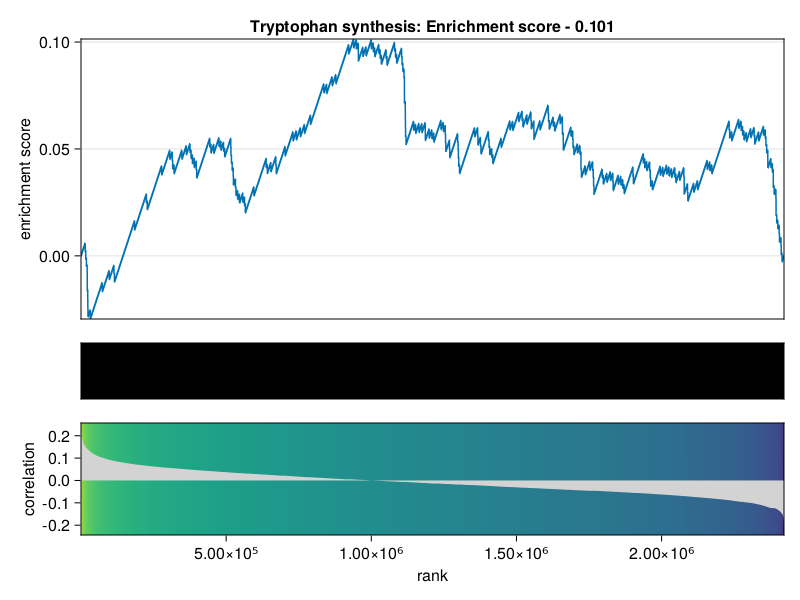
\includegraphics[width=1\linewidth]{../figures/fsea_Tryptophan-synthesis.png}
        \end{figure}

    \end{columns}

\end{frame}

\begin{frame}{SAM synthesis}
    \begin{columns}[c] % The "c" option specifies centered vertical alignment while the "t" option is used for top vertical alignment

        \column{.7\textwidth} % Right column and width
        \begin{figure}
            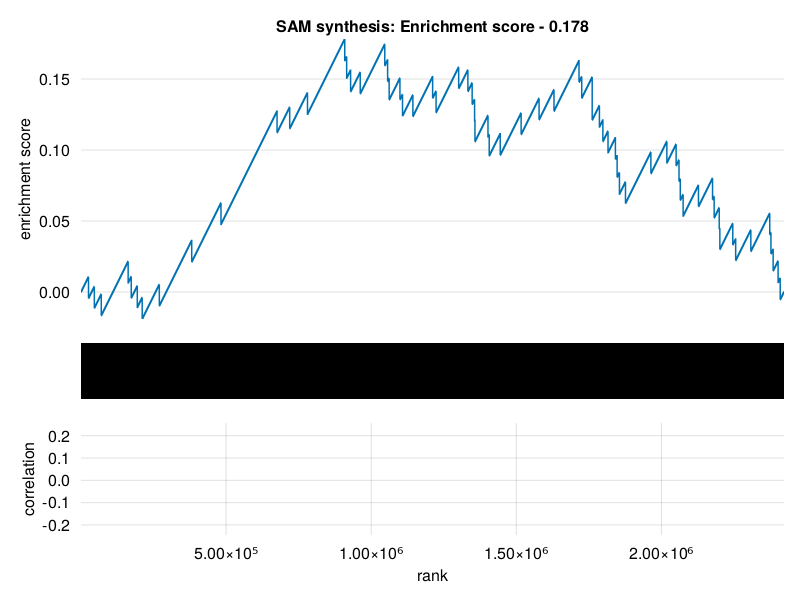
\includegraphics[width=1\linewidth]{../figures/fsea_SAM-synthesis.png}
        \end{figure}

    \end{columns}

\end{frame}

\begin{frame}{p-Cresol synthesis}
    \begin{columns}[c] % The "c" option specifies centered vertical alignment while the "t" option is used for top vertical alignment

        \column{.7\textwidth} % Right column and width
        \begin{figure}
            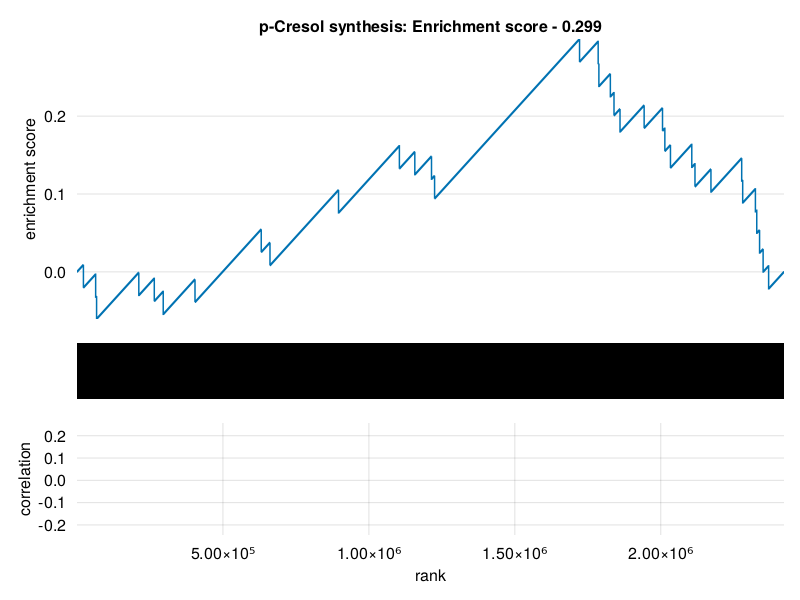
\includegraphics[width=1\linewidth]{../figures/fsea_p-Cresol-synthesis.png}
        \end{figure}

    \end{columns}

\end{frame}

\begin{frame}{Acetate synthesis}
    \begin{columns}[c] % The "c" option specifies centered vertical alignment while the "t" option is used for top vertical alignment

        \column{.7\textwidth} % Right column and width
        \begin{figure}
            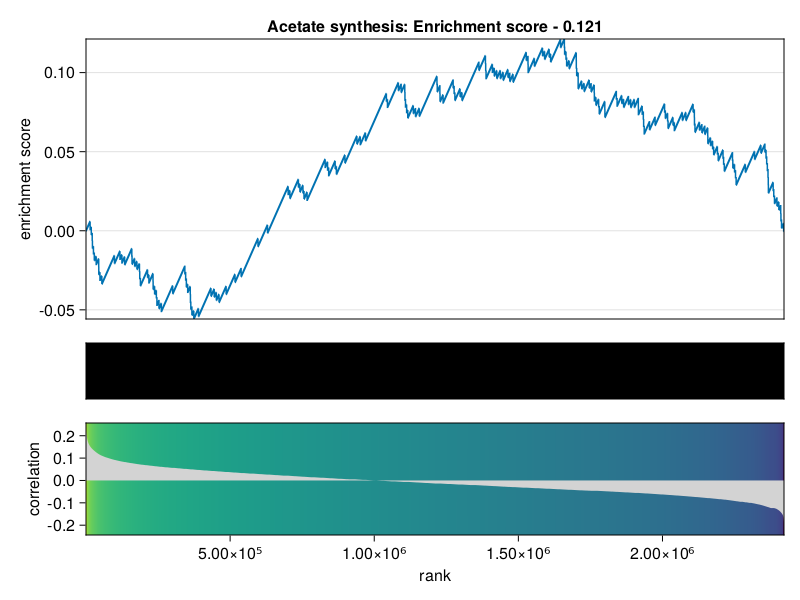
\includegraphics[width=1\linewidth]{../figures/fsea_Acetate-synthesis.png}
        \end{figure}

    \end{columns}

\end{frame}

\begin{frame}{Quinolinic acid degradation}
    \begin{columns}[c] % The "c" option specifies centered vertical alignment while the "t" option is used for top vertical alignment

        \column{.7\textwidth} % Right column and width
        \begin{figure}
            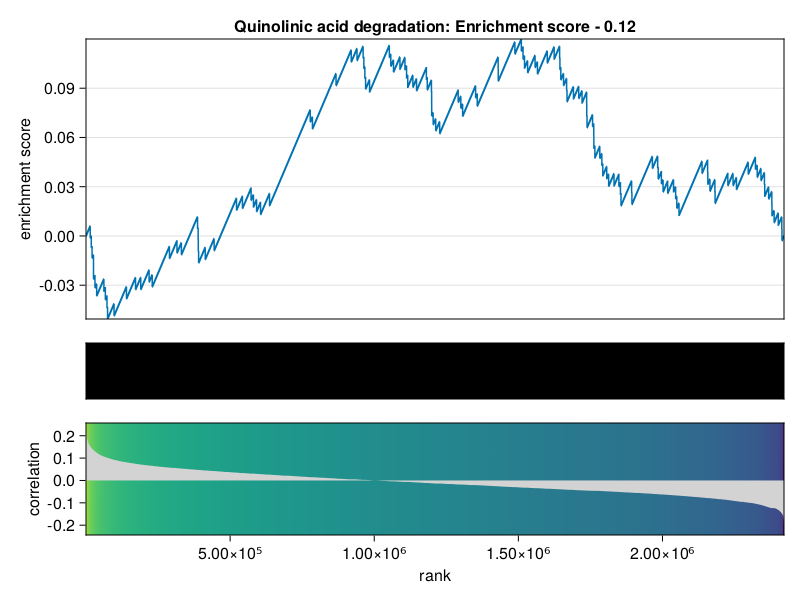
\includegraphics[width=1\linewidth]{../figures/fsea_Quinolinic-acid-degradation.png}
        \end{figure}

    \end{columns}

\end{frame}

\begin{frame}{Butyrate synthesis}
    \begin{columns}[c] % The "c" option specifies centered vertical alignment while the "t" option is used for top vertical alignment

        \column{.7\textwidth} % Right column and width
        \begin{figure}
            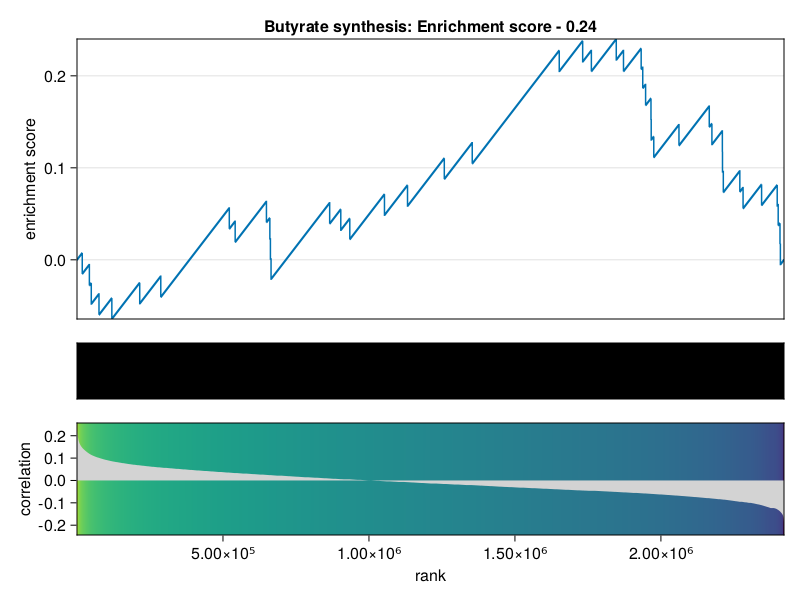
\includegraphics[width=1\linewidth]{../figures/fsea_Butyrate-synthesis.png}
        \end{figure}

    \end{columns}

\end{frame}
